\documentclass[12pt]{article}
\usepackage[utf8]{inputenc}
\usepackage{cite}
\usepackage[spanish]{babel}
\selectlanguage{spanish}
\usepackage{graphicx}
\graphicspath{ {files/} }
\usepackage{url}
\usepackage{natbib}
\usepackage{amsmath}
\usepackage{paracol}
\usepackage{tensor}
\usepackage{float}




\title{Reporte sobre la Actividad 9}
\author{García Parra Pedro}
\date{Mayo 2019}

\begin{document}

\maketitle

En esta actividad se nos pide dar soluci\'on a un sistema f\'isico resolviendo una eciaci\'on diferencial de segundo orden. El sistema a resolver (\textit{figura \ref{fig:prob}}) est\'a compuesto como: dos masas sostenidas por tres resortes, el primer resorte, de constante el\'astica $k_1$ y longitud $L_1$ se sostiene de la pared y de una de las masas, el segundo resorte, de constante el\'astica $k_2$ y longitud $L_2$ sostiene a ambas masas de su extremo, el tercer resorte, de constante el\'astica $k_3$ y longitud $L_3$ sostiene a la segunda masa y a la pared.

\begin{figure}
    \centering
    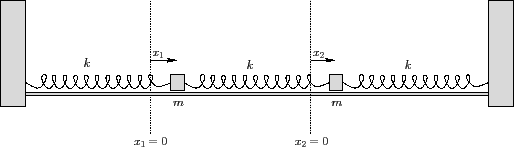
\includegraphics[scale = 0.7]{problema.png}
    \caption{Imagen del sistema f\'isico a resolver. Dos masas sostenidas por tres resortes.}
    \label{fig:prob}
\end{figure}

Antes de resolver este sistema observamos otro sistema un poco m\'as sencillo ya resuelto.
Este sistema (\textit{figura \ref{fig:ejemplo}}) se compone de dos masas, $m_1$ y $m_2$, sostenidas por dos resortes; el primer resorte, con constante elastica $k_1$ y longitud $L_1$ esta agarrado de una pared y sostiene a una de las masas por su extremo, el segundo resorte, de constante elastica $k_2$ y longitud $L_2$, sostiene a ambas masas . Las ecuaciones diferenciales del sistema son:
$$ m_1x''_1+b_1x'_1+k_1(x_1-L_1)-k_2(x_2-x_1-L_2)=0 $$
$$ m_2x''_2+b_2x'_2+k_2(x_2-x_1-L_2)=0 $$

Este problema est\'a resuelto utilizando la funcion \texttt{odeint} de la libreria de \textit{scipy}.
Como las ecuaciones son de segundo orden primero debemos hacer algo para que el resolvedor ODE de python pueda solucionarlas.
Se definiran dos variables:
$$ y_1 = x'_1 $$
$$ y_2 = x'_2 $$
As\'i podemos escribir las ecuaciones anteriores como:
\begin{equation*}
    \begin{split}
        x'_1&=y_1 \\
        y'_1&=(-b_1y_1-k_1(x_1-L_1)+k_2(x_2-x_1-L_2))/m_1\\
        x'_2&=y_2\\
        y'_2&=(-b_2y_2-k_2(x_2-x_1-L_2))/m_2
    \end{split}
\end{equation*}

Estas ecuaciones ahora pueden ser resuelatas por \textit{scipy}.
\begin{figure}
    \centering
    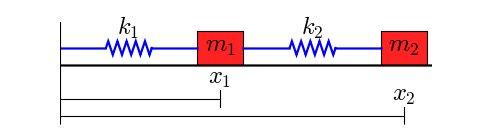
\includegraphics[scale = 0.8]{prob_simple.png}
    \caption{Segundo sistema f\'isico. Dos masas sostenidas por dos resortes.}
    \label{fig:ejemplo}
\end{figure} \\
\\
Ahora para resolver el sistema de tres resortes añadiremos un tercer resorte a las ecuaciones planteadas anteriormente. Este termino deber\'a contener la constante de elastisidad $k_3$ del resorte de longitud $L_3$. Este termino ser\'a $-k_3(-x_2 + (L_1+ L_2))$, este t\'ermino mide la fuerza con la cual el resorte 3 \textit{jala} a la masa 3. Tras agregar este t\'ermino las ecuaciones quedan como:
\begin{equation*}
    \begin{split}
        x'_1&=y_1 \\
        y'_1&=(-b_1y_1-k_1(x_1-L_1)+k_2(x_2-x_1-L_2 ))/m_1\\
        x'_2&=y_2\\
        y'_2&=(-b_2y_2-k_2(x_2-x_1-L_2) - k_3(-x_2 + (L_1+ L_2)))/m_2
    \end{split}
\end{equation*}
De igual manera seutiliza la funcion \texttt{odeint} de la librer\'ia \textit{scipy} para resolver estas ecuaciones diferenciales. La \textit{figura \ref{fig:solucion}} muestra una gr\'afica realizada con las soluciones para la posici\'on de las masas.
\begin{figure}
    \centering
    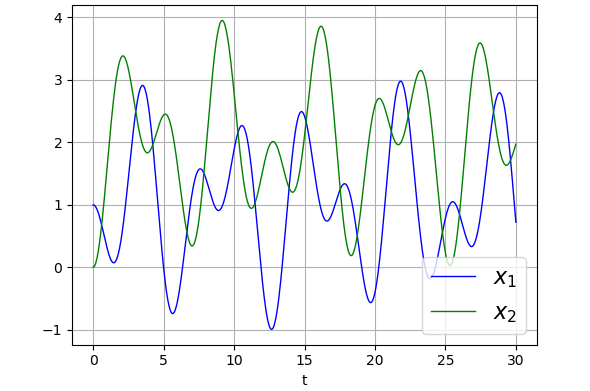
\includegraphics[scale = 0.8]{two_springs.png}
    \caption{Grafica del desplazamiento de ambas masas. Soluci\'on a las ecuaciones diferenciales del sistema de tres resortes.}
    \label{fig:solucion}
\end{figure}

\end{document}
